<<<<<<< .mine
%%==================================================================%%
%% Author : Perez Ruiz, Alejandro                                   %%
%% Author : Pablo S�nchez                                           %%
%% Version: 1.1, 13/06/2011                                         %%
%%                                                                  %%
%% Memoria del Proyecto Fin de Carrera                              %%
%% Cap�tulo Planificacion, Archivo ra�z                             %%
%%==================================================================%%
=======
%%=================================================================%%
%% Author : Perez Ruiz, Alejandro                                  %%
%% Author : Pablo S�nchez                                          %%    
% Version: 1.0, 16/03/2011                                         %%                                                                                    %                                                                  %%
% Memoria del Proyecto Fin de Carrera                              %%
% Cap�tulo Planificacion, Archivo ra�z                             %%
%==================================================================%%
>>>>>>> .r383

\chapterheader{Definici�n y Planificaci�n del Proyecto}{Definici�n y Planificaci�n del Proyecto}
\label{chap:planificacion}

El presente cap�tulo describe el caso de estudio cuyo desarrollo es el objetivo del presente proyecto, as� como la metodolog�a seguida para la realizaci�n del mismo. Se presenta tambi�n una descripci�n general de las etapas inicialmente planificadas, de acuerdo con la metodolog�a escogida, para el correcto desarrollo del proyecto.

\chaptertoc

\section{Caso de Estudio: Hogares Inteligentes Automatizados}

<<<<<<< .mine
%%==================================================================%%
%% Author : Abascal Fern�ndez, Patricia                             %%
%%          S�nchez Barreiro, Pablo                                 %%
%% Version: 1.1, 17/04/2013                                         %%
%%                                                                  %%
%% Memoria del Proyecto Fin de Carrera                              %%
%% Planificacion/CasoEstudio                                        %%
%%==================================================================%%

El objetivo �ltimo del presente proyecto es la construcci�n de una l�nea de productos software sobre la plataforma .NET para hogares automatizados y/o inteligentes.

El objetivo de estos hogares es aumentar la comodidad y seguridad de sus habitantes, as� como hacer un uso m�s eficiente de la energ�a consumida. Los ejemplos m�s comunes de tareas automatizadas dentro de un hogar inteligente son el control de las luces, ventanas, puertas, persianas, aparatos de fr�o/calor, as� como otros dispositivos, que forman parte de un hogar. Un hogar inteligente tambi�n busca incrementar la seguridad de sus habitantes mediante sistemas automatizados de vigilancia y alerta de potenciales situaciones de riesgo. Por ejemplo, el sistema deber�a encargarse de detecci�n de humos o de la existencia de ventanas abiertas cuando se abandona el hogar.

El funcionamiento de un hogar inteligente se basa en el siguiente esquema: (1) el sistema lee datos o recibe datos de una serie de sensores; (2) se procesan dichos datos; y (3) se activan los actuadores para realizar las  acciones que correspondan en funci�n de los datos recibidos de los sensores.

Todos los sensores y actuadores se comunican a trav�s de un dispositivo especial denominado puerta de enlace (\emph{Gateway}, en ingl�s). Dicho dispositivo se encarga de coordinar de forma adecuada los diferentes dispositivos existentes en el hogar, de acuerdo a los par�metros y preferencias especificados por los habitantes del mismo. Los habitantes del hogar se comunicar�n con la puerta de enlace a trav�s de una interfaz gr�fica.
Este proyecto tiene como objetivo el desarrollo de un hogar inteligente como una l�nea de productos software, con un n�mero variable de plantas y habitaciones. El n�mero de habitaciones por planta es tambi�n variable. La l�nea de productos deber� ofrecer varios servicios, que podr�n ser opcionalmente incluidos en la instalaci�n del software para un un hogar determinado. Dichos servicios se clasifican en funciones b�sicas y complejas, las cuales describimos a continuaci�n.

\paragraph{Funciones b�sicas} \ \\

\begin{enumerate}
\item \emph{Control autom�tico de luces:} Los habitantes del hogar deben ser capaces de encender, apagar y ajustar la intensidad de las diferentes luces de la casa. El n�mero de luces por habitaci�n es variable. El ajuste debe realizarse especificando un valor de intensidad.
\item \emph{Control autom�tico de ventanas:} Los residentes tienen que ser capaces de controlar las ventanas autom�ticamente. De tal modo que puedan indicar la apertura de una ventana desde las interfaces de usuario disponibles.
\item \emph{Control autom�tico de persianas:} Los habitantes podr�n subir y bajar las persianas de las ventanas de manera autom�tica.
\item \emph{Control autom�tico de temperatura:} El usuario ser� capaz de ajustar la temperatura de la casa. La temperatura se medir� siempre en grados celsius.
\end{enumerate}

\paragraph{Funciones complejas} \ \\

\begin{enumerate}
\item \emph{Control inteligente de energ�a:} Esta funcionalidad trata de coordinar el uso de ventanas y aparatos de fr�o/calor para regular la temperatura interna de la casa de manera que se haga un uso m�s eficiente de la energ�a. Por ejemplo, si se recibe la orden de calentar la casa, a la vez que se activan los radiadores se cerrar�n las ventanas para evitar las p�rdidas de calor.
\item \emph{Presencia simulada:} Para evitar posibles robos, cuando los habitantes abandonen la casa por un periodo largo de tiempo, se deber� poder simular la presencia de personas en las casas. Hay dos opciones de simulaci�n (no exclusivas):
	\begin{enumerate}
	\item \emph{Simulaci�n de las luces:} Las luces se deber�n apagar y encender para simular la presencia de habitantes en la casa.
	\item \emph{Simulaci�n de persianas:} Las persianas se deber�n subir y bajar autom�tica para simular la presencia de individuos dentro de la casa.
	\end{enumerate}
\end{enumerate}

Todas estas funciones son opcionales. Las personas interesadas en adquirir el sistema podr�n incluir en una instalaci�n concreta de este software el n�mero de funciones que ellos deseen. La siguiente secci�n profundiza en el concepto \emph{l�nea de productos software}. 
=======
El objetivo de estos hogares es el aumento de la comodidad y seguridad de sus habitantes, as� como hacer un uso m�s eficiente de la energ�a consumida. Se ha elegido este dominio por ser un dominio donde el uso de un enfoque basado en L�neas de Productos Software se hace casi imperativo, debido a la gran variabilidad existente en estos productos. Esta variabilidad se debe tanto a motivos de hardware, dado que los dispositivos a ser controlados e interconectados pueden variar enormemente, como funcionales, dado que existen multitud de funcionalidades que se pueden ofrecer de manera opcional o alternativa al usuario, no siendo necesario que un determinado hogar las posea todas ellas.
>>>>>>> .r383

\section{Metodolog�a de Desarrollo}

%%==================================================================%%
%% Author : Perez Ruiz, Alejandro                                   %%
%% Author : Pablo S�nchez                                           %%
%% Version: 1.1, 13/06/2011                                         %%
%%                                                                  %%
%% Memoria del Proyecto Fin de Carrera                              %%
%% Cap�tulo Planificacion/Metodolog�a                               %%
%%==================================================================%%

El primer paso para la correcta realizaci�n de todo proyecto software es elegir la metodolog�a de desarrollo que mejor se adec�e a las caracter�sticas de dicho proyecto. Dicha metodolog�a se ha elegido de entre las conocidas como  \emph{�giles}~\cite{cockburn:2001}, al entender que por el tama�o del proyecto y la necesidad de cierta flexibilidad en su desarrollo de sus requisitos, son las que mejor se adaptan a las particularidades de nuestro proyecto. Dentro de las metodolog�as �giles, existen dos que, por sus caracter�sticas, parecen adecuarse mejor al desarrollo de l�neas de productos software: (1) el \emph{Desarrollo Dirigido por Caracter�sticas} y (2) el \emph{Desarrollo Dirigido por Casos de Prueba}. A continuaci�n, describimos brevemente las siguientes subsecciones describe ambos procesos.

\subsection{Desarrollo Dirigido por Caracter�sticas}

La \emph{metodolog�a de Desarrollo Dirigido por Caracter�sticas}~\cite{palmer:2002} (\emph{FDD}, por su nombre en ingl�s \emph{Feature-Driven Development}) es un proceso �gil que se basa en construir iteraciones cortas que produzcan incrementos funcionales en el software que los clientes y personas encargadas de la gesti�n del proyecto puedan ver, analizar y aprobar.

En cada iteraci�n se trata de construir una \emph{caracter�stica}, definida como un incremento en la funcionalidad de un producto con significado para el cliente~\cite{batory:2005:propositional}. Esta metodolog�a de desarrollo consiste en cinco procesos secuenciales, los cuales se citan a continuaci�n:

\begin{enumerate}
	%%==================================================================%%
	%% HECHO(Pablo): Esto del modelo general no entiendo lo que es.      %%
	%%     Si te refieres a la arquitectura general del sistema,        %%
	%%     cambialo por "Especificaci�n de la arquitectura global del   %%
	%%      sistema                                                     %%
	%%==================================================================%%
	%%==================================================================%%
	%% HECHO(Pablo): �No habr�a que cambiar el punto 1 y 2 de orden?     %%
	%%==================================================================%%
	\item Especificaci�n de la arquitectura global del sistema.
	\item Construcci�n de la lista de caracter�sticas (en ingl�s, \emph{features}) que componen el sistema.
	\item Planificaci�n por caracter�stica.
	\item Dise�o por caracter�stica.
	\item Construcci�n por caracter�stica.
\end{enumerate}

La principal ventaja de esta metodolog�a es que est� orientada y gobernada por caracter�sticas, que son un concepto clave en el desarrollo de l�neas de productos software.

%%==========================================================================%%
%% NOTA(Pablo): Esto me gusta porque se ve que hay un proceso de trabajo    %%
%%              detr�s y no has cogido la primera metodolog�a que te ha     %%
%%              apetecido. No obstante, si la memoria se hace muy larga,    %%
%%              lo quitamos.                                                %%        %%==========================================================================%%

\subsection{Desarrollo Dirigido por Casos de Pruebas}

El \emph{Desarrollo Dirigido por Casos de Pruebas} (\emph{TDD}, por su nombre en ingl�s \emph{Test Driven Development})~\cite{astels:2003} es un proceso �gil, iterativo e incremental, en el que el sistema se desarrolla para satisfacer unos casos de prueba bien definidos antes de construir cada iteraci�n.

El primer paso a realizar de acuerdo con esta metodolog�a es definir una lista de requisitos. A continuaci�n, se aplica el siguiente proceso de forma iterativa hasta completar el proyecto:

\begin{enumerate}
	\item Seleccionar uno o m�s requisitos.
	\item Escribir casos de prueba que verifiquen que dichos requisitos se satisfacen .
	\item Desarrollar el sistema de la forma m�s sencilla posible para pasar los casos de prueba.
	\item Verificar que el conjunto de pruebas funciona correctamente.
	\item Refactorizar la soluci�n desarrollada en caso de que fuese necesario.
	\item Actualizar la lista de requisitos.
\end{enumerate}

Este proceso tiene dos importantes virtudes: (1) est� muy orientada a satisfacer los requisitos; y (2) genera software fiable, si los casos de prueba est�n bien dise�ados. Al desarrollar el software por grupos de requisitos, podr�a considerarse que en cierto modo est� orientado o dirigido por caracter�sticas.

Sin embargo, el concepto de caracter�stica, elemento clave de una l�nea de productos software, no es un elemento tan central en la metodolog�a, tal como ocurr�a en el caso de la metodolog�a anterior. Por tanto, para el desarrollo del presente proyecto seguiremos una metodolog�a �gil dirigida por caracter�sticas.

%%==========================================================================%%
%% NOTA(Pablo): Esto queda demasiado largo y tampoco aporta informaci�n     %%
%%              vital, as� que lo suprimimos                                %%       %%==========================================================================%%
%%
%% \subsubsection{Elecci�n del proceso}
%% Debido a que el proceso \emph{Feature Driven Development} est� especialmente
%% orientado para proyectos que se pueden descomponer f�cilmente en
%% caracter�sticas, se ha seleccionado para utilizarlo como proceso de
%% desarrollo. Como es f�cilmente visible el presente proyecto debe ser
%% descompuesto en sus diferentes caracter�sticas y/o tareas para llevar a cabo
%% su implementaci�n. Adem�s, dichas caracter�sticas deben estar lo
%% suficientemente encapsuladas para poder componerlas y crear diferentes
%% configuraciones para el amplio abanico de posibles hogares inteligentes. De
%% tal modo, que es de vital importancia seguir un proceso de desarrollo que se
%% oriente hacia la descomposici�n de caracter�sticas, tal y como hace
%% \emph{Feature Driven Development}.
%%
%%==========================================================================%%

La siguiente secci�n describe la planificaci�n general creada para la realizaci�n del proyecto de acuerdo a la metodolog�a escogida.



\section{Planificaci�n del Proyecto}

%%==================================================================%%
%% Author : Perez Ruiz, Alejandro                                   %%
%% Author : Pablo S�nchez                                           %%
%% Version: 1.1, 13/06/2011                                         %%
%%                                                                  %%
%% Memoria del Proyecto Fin de Carrera                              %%
%% Cap�tulo Planificacion/Planificacion                             %%
%%==================================================================%%

Esta secci�n describe la planificaci�n general (definici�n de etapas, objetivos de cada etapa, secuenciaci�n de etapas, etc.) seguida para la realizaci�n del presente proyecto.

Cabe recordar que en nuestro caso, al estar desarrollando una l�nea de productos software, habr� que realizar dos tipos de proyectos: (1) el desarrollo de la familia de productos, de forma que mediante composici�n de caracter�sticas se puedan obtener productos software pertenecientes a dicha familia; y (2) el desarrollo de los mecanismos necesarios para que la creaci�n de productos espec�ficos a partir de la infraestructura creada en el punto anterior sea lo m�s autom�tica posible. A continuaci�n describimos por separado la planificaci�n para cada una de ellas.

\subsection{Planificaci�n para la Fase de Ingenier�a del Dominio}

%%====================================================================%%
%% NOTA(Pablo): Las restricciones no se leen bien y habr�a que hacer  %%
%%              esta figrua m�s compacta                              %%
%%====================================================================%%

\begin{figure}[!tb]
  % Requires \usepackage{graphicx}
  \centering 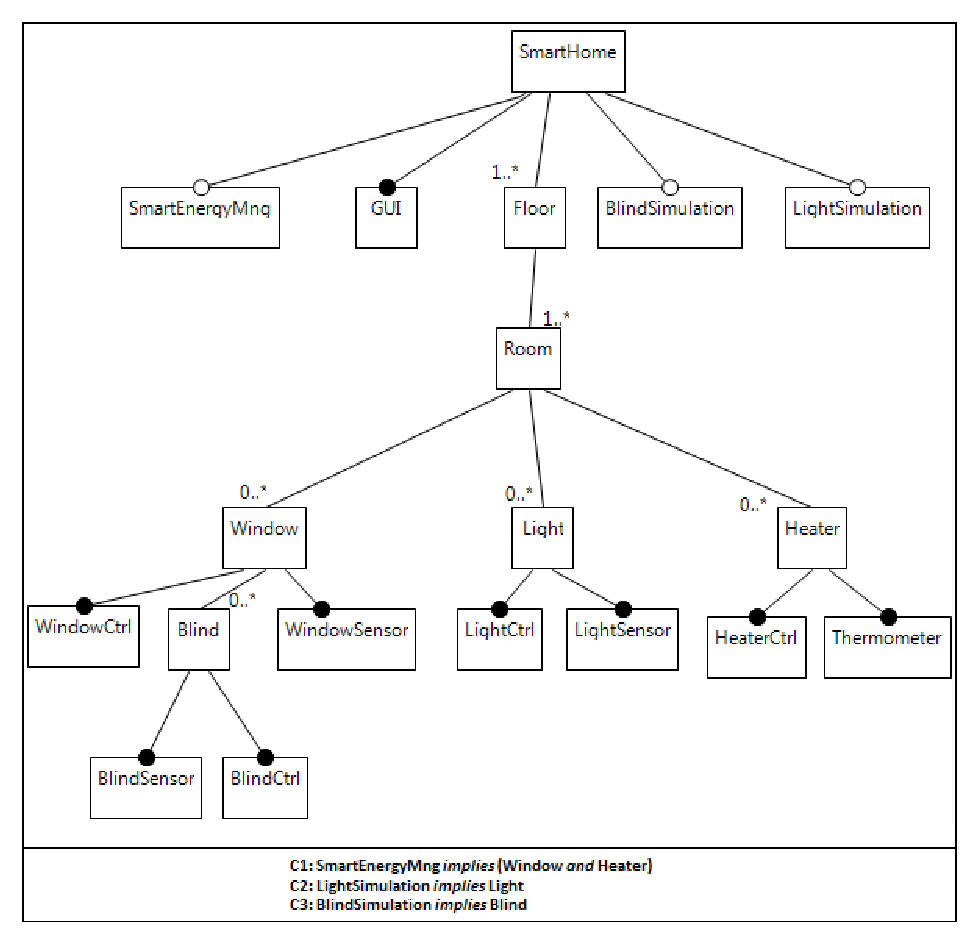
\includegraphics[width=.85\linewidth]{planificacion/images/featureModelReal.eps} \\
  \caption{Diagrama de caracter�sticas para un hogar inteligente}
  \label{plan:fig:modelReal}
\end{figure}


De acuerdo a la metodolog�a de desarrollo �gil dirigida por caracter�sticas, la primera tarea a realizar para construir nuestra familia de productos software
es identificar y especificar cuales son las diferentes caracter�sticas que forman parte de dicha familia. Por tanto, para completar esta primera etapa, se crea el �rbol de caracter�sticas (cf. Secci�n~\ref{back:sec:feature}) que se muestra en la Figura~\ref{plan:fig:modelReal}.

Dicho �rbol de caracter�sticas especifica que todo hogar inteligente debe tener al menos una planta y una habitaci�n por planta. Cada habitaci�n puede tener instaladas diferentes funcionalidades, tales como control autom�tico de ventanas, de luces, de aparatos de fr�o/calor o de persianas. A nivel global, y como caracter�sticas opcionales, se puede decidir instalar la funci�n para la gesti�n inteligente de la energ�a (\imp{SmartEnergyMng}).

Recordemos que esta funci�n se encarga de gestionar de forma coordinada las ventanas y los aparatos de fr�o/calor del hogar para fomentar el ahorro de energ�a. Por lo tanto, esta funcionalidad requiere que al menos la funci�n de control de los aparatos de fr�o/calor m�s el control autom�tico de ventanas haya sido seleccionado para al menos una habitaci�n de la casa.
%%==================================================================%%
%% NOTA(Pablo): En realidad esa restricci�n no expresa eso.         %%
%%              As� que no la pongas en la figura, sino que         %%
%%              simplemente la describes con palabras               %%
%%              (Acuerdate del art�culo del SPLC 2011)              %%
%%==================================================================%%
% Dicha dependencia se especifica a trav�s de la la restricci�n C1
% de la Figura~\ref{plan:fig:modelReal}.
%%==================================================================%%

Algo similar acontece con la simulaci�n de las luces (\emph{LightSimulation}) y de las persianas (\emph{BlindSimulation}). Como es obvio, la simulaci�n de luces requiere que el control autom�tico de luces  haya sido incluido en al menos una habitaci�n de la casa. La simulaci�n de persianas requiere lo mismo, pero para el control autom�tico de persianas.

Usando el �rbol de la Figura~\ref{plan:fig:modelReal}, decidimos desarrollar el proyecto por incrementos basados en el n�mero de servicios que pueden incluirse en un hogar inteligente. Por tanto, el proceso de desarrollo de nuestro proyecto comprender� 8 iteraciones, en cada una de las cuales se desarrollar� un nuevo servicio. Dichas iteraciones se citan a continuaci�n:

\begin{enumerate}
	\item Desarrollo de la arquitectura b�sica del sistema (\imp{BaseSystem}).
	\item Desarrollo de los servicios de control de aparatos de fr�o/calor
		(\imp{HeaterMng}).
	\item Desarrollo de los servicios de control de ventanas (\imp{WindowMng}).
	\item Desarrollo de los servicios de control inteligente de la energ�a (\imp{SmartenergyMng}).
	\item Desarrollo de los servicios de control de persianas
		(\imp{BlindMng}).
	\item Desarrollo de los servicios de control autom�tico de luces
		(\imp{LightMng}).
	\item Desarrollo de los servicios de simulaci�n de luces
		(\imp{LightSimulation}).
	\item Desarrollo de los servicios de simulaci�n de persianas
		(\imp{BlindSimulation}).
\end{enumerate}

%%========================================================================%%
%% NOTA(Pablo): En realidad el diagram de Gannt no me convence.           %%
%% Perfer�a simplemente un grafo de dependencias.
%%========================================================================%%
La Figura~\ref{plan:fig:gantt} muestra las dependencias y secuenciaci�n de dichas tareas.

%%========================================================================%%
%% NOTA(Pablo): Lo de los dos diagramas queda confuso y demasiado largo   %%
%%========================================================================%%
%%
%% \begin{figure}[!tb]
%%  % Requires \usepackage{graphicx}
%%  \centering
%%
%% %% \includegraphics[width=.85\linewidth]
%% {planificacion/images/featureModelSimplificado.eps} \\
%%  \caption{Diagrama de caracter�sticas para un hogar inteligente simplificado}
%%  \label{plan:fig:modelSimplificado}
%% \end{figure}
%%
%%========================================================================%%

Una vez extra�das y secuenciadas las caracter�sticas de nuestra familia de productos software, el siguiente paso es extraer los requisitos de alto nivel para nuestra familia de productos y asociarlos a cada caracter�sticas. Los requisitos de alto nivel del sistema y su correspondencia con las caracter�sticas de la familia de productos se muestran en la Tabla~\ref{plan:table:requisitos}.

\begin{table}[!tb]
  % Requires \usepackage{graphicx}
  \centering 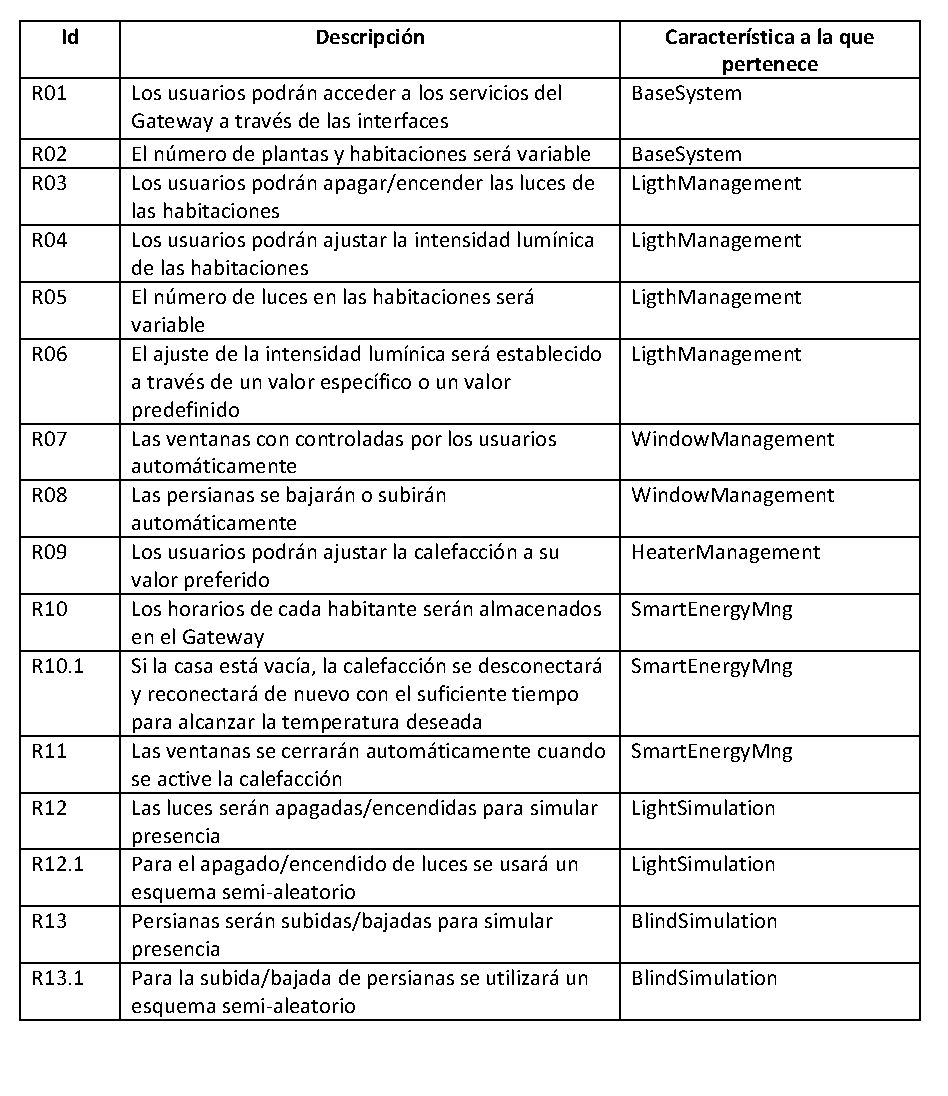
\includegraphics[width=.85\linewidth]{planificacion/images/requisitosTabla.eps} \\
  \caption{Correspondencia entre los requisitos de alto nivel y las caracter�sticas.}
  \label{plan:table:requisitos}
\end{table}

Una vez realizada esta correspondencia, s�lo quedar� realizar las 8 iteraciones, incluyendo las siguientes etapas por cada fase:

\begin{enumerate}
	\item Refinamiento de requisitos.
	\item Dise�o software. Se usar� UML como lenguaje de modelado.
	\item Dise�o de la interfaz gr�fica.
	\item Implementaci�n.
	\item Pruebas.
\end{enumerate}

Una vez concluidas las 8 iteraciones, se proceder� a la creaci�n de la infraestructura necesaria para crear productos concretos acordes a las necesidades de cada usuarios.

\subsection{Planificaci�n para la Fase de Ingenier�a de la Aplicaci�n}

%%========================================================================%%
%% NOTA(Pablo): Esto ahora es redundante                                  %%
%%========================================================================%%
%
% Como ya se coment� en el Cap�tulo \ref{chap:background}, los proyectos que
% desarrollan una l�nea de productos software se descomponen en dos fases
% denominadas ingenier�a de dominio(\emph{Domain Engineering}, en ingl�s) e
% ingenier�a de aplicaci�n(\emph{Application Engineering}, en ingl�s), en el
% primero de ellos se va a desarrollar la infraestructura necesaria para
% construir el sistema espec�fico, mientras que la ingenier�a de aplicaci�n
% utilizar� esta infraestructura para crear aplicaciones espec�ficas. Por ello,
% lo primero que se debe llevar a cabo es la fase de ingenier�a de dominio, que
% consiste en implementar todas las caracter�sticas y requisitos descritos
% anteriormente.
%
%%========================================================================%%

Una vez creada la familia de productos, la siguiente fase consiste en generar
la infraestructura que permita crear productos espec�ficos, tan f�cil como sea posible, mediante la composici�n de las caracter�sticas creadas en el punto anterior.

%%========================================================================%%
%% NOTA(Pablo): Esto ahora sobra                                          %%      %%========================================================================%%
%%
%% Por lo tanto, la figura \ref{plan:fig:gantt} muestra la secuenciaci�n
%% de las distintas tareas/caracter�sticas, a trav�s de un diagrama de
%% Gantt que se deben desarrollar para completar la fase de ingenier�a de
%% dominio. En la figura se describe cuales son las dependencias de las
%% tareas y el orden en el que se deben desarrollar. Las dependencias
%% surgen de las restricciones mostradas en la figura
%% \ref{plan:fig:modelSimplificado}.
%%
%% \begin{figure}[!tb]
%% % Requires \usepackage{graphicx}
%% \centering 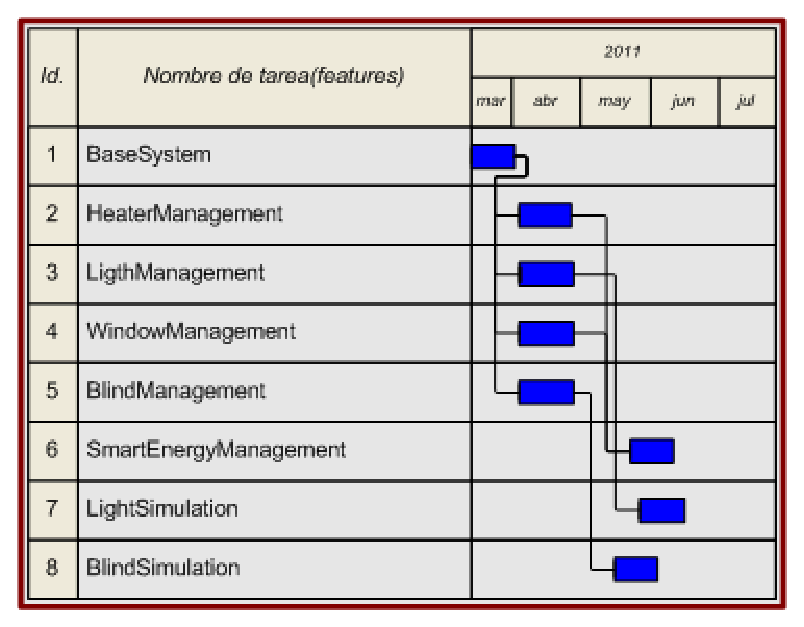
\includegraphics{planificacion/images/gantt.eps} \\
%% \caption{Diagrama de Gantt que muestra las dependencias entre
%%          tareas para la ingenier�a de dominio}
%% \label{plan:fig:gantt}
%% \end{figure}
%%
%% De este modo y teniendo como referencia el proceso de desarrollo software
%% seleccionado, por cada caracter�stica mostrada en el diagrama de Gantt se
%% dise�a la caracter�stica,se construye y se prueba. Adem�s por cada una de
%% estas caracter�sticas se implementar� su interfaz gr�fica correspondiente por %% lo que %% en cada una de ellas se suma la tarea de dise�o, construcci�n y
%% pruebas.
%%
%% Una vez desarrolladas todas las caracter�sticas se puede dar por concluida la %% fase de ingenier�a de dominio, por lo que se procede a describir la
%% planificaci�n de la fase siguiente,la ingenier�a de aplicaci�n.
%%========================================================================%%

Con el objeto de hacer la fase de Ingenier�a de la Aplicaci�n lo m�s autom�tica posible, utilizaremos t�cnica de desarrollo software dirigido por modelos~\cite{beydeda:2005}. M�s concretamente, usaremos generaci�n de c�digo a partir de lenguajes espec�ficos de dominio (\emph{DSL} por sus nombre en ingl�s (Domain Specific Language))~\cite{kleppe:2008,kelly:2008}.

La idea es que el desarrollador use un lenguaje espec�fico de dominio para modelar el hogar automatizado que mejor se adapte a las necesidades de un cliente espec�fico. A partir de dicho modelo, se generar� de forma autom�tica el c�digo necesario para componer las caracter�sticas creadas en la fase de Ingenier�a del Dominio, y derivar as� un producto concreto. Para implementar esta fase usaremos el entorno de desarrollo software dirigido por modelos proporcionado por Visual Studio 2010 denominado DSL Tools~\cite{cook:1990}. 

\begin{figure}[!tb]
  % Requires \usepackage{graphicx}
  \centering 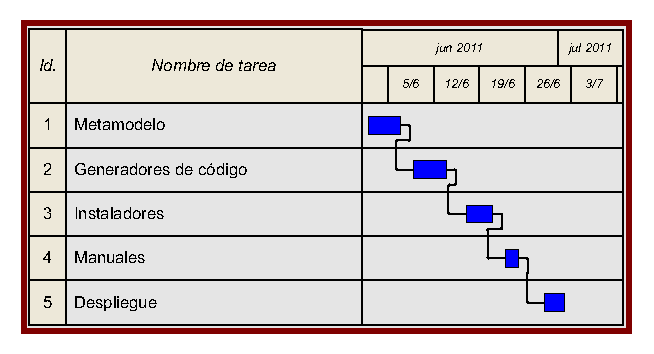
\includegraphics{planificacion/images/ganttApplication.eps} \\
  \caption{Diagrama de Gantt que muestra las dependencias entre tareas para la ingenier�a de aplicaci�n}
  \label{plan:fig:ganttApplication}
\end{figure}

%%========================================================================%%
%% NOTA(Pablo): En realidad el diagram de Gannt no me convence.           %%
%% Perfer�a simplemente un grafo de dependencias.
%%========================================================================%%
Las etapas a realizar para la construcci�n de dicho DSL y su generador de c�digo asociado, de acuerdo al proceso habitual de la ingenier�a de lenguajes dirigidos por modelos~\cite{kleppe:2008}, son las que se enumeran a continuaci�n, y se reflejan en la Figura~\ref{plan:fig:ganttApplication}:

\begin{enumerate}
	\item En primer lugar es necesario desarrollar un metamodelo, o gram�tica, para nuestro lenguaje de modelado.A continuaci�n, usando las DSL Tools, se generar� autom�tica un \emph{plugin} para Visual Studio 2010 que permita la edici�n de dichos modelos. Este plugin permitir� al construcci�n de modelos de hogares inteligentes concretos que satisfagan las necesidades particulares de cada usuario.
	\item A continuaci�n,  se desarrollar�n los generadores de c�digo para la composici�n autom�tica de as diferentes caracter�sticas que deben integrar el software para un hogar concreto a partir de un modelo creado haciendo uso del \emph{plugin} para Visual Studio creado en el punto anterior.
	\item Con lo anterior, ya tenemos la infraestructura para derivar autom�ticamante productos concretos mediante la composici�n de caracter�sticas. Por tanto, el siguiente fase ser�a el despliegue de nuestro producto. En dicha fase se realizar�n las siguientes actividades:
		\begin{enumerate} 
			\item Se crear�n instaladores que permitan utilizar todo lo construido hasta este momento en cualquier computar provisto del entorno Visual Studio 2010.
			\item Para facilitar el uso del producto, se crear�n una serie de manuales de usuario.
			\item Para darle visibilidad y difusi�n al proyecto, se crear� una p�gina web para el mismo. De dicha p�gina web se podr�n descargar tanto los instaladores como los manuales. Adem�s, en dicha p�gina se incluir�n los manuales de usuario, as� como diverso material de promoci�n del proyecto, como proyectos relacionados, publicaciones, v�deos mostrando el funcionamiento de la herramienta, etc.
		\end{enumerate}
\end{enumerate}

%%=============================================================================================================%%
%% NOTA(Pablo): En realidad en estos caso las fases de implementaci�n y pruebas no est�n tan claras            %%
%%=============================================================================================================%%
%%
%% Tal y como ha ocurrido en la fase de ingenier�a de dominio cada tarea de la figura 
%% \ref{plan:fig:ganttApplication} es considerada como una caracter�stica, por lo que siguiendo el proceso de 
%% desarrollo software elegido, por cada tarea se realizar� su dise�o, construcci�n y respectivas pruebas.
%%
%%=============================================================================================================%%

\section{Sumario}

En este cap�tulo se ha descrito el caso de estudio de los hogares inteligentes, posteriormente se han estudiado algunos procesos de desarrollo software para realizar la planificaci�n del proyecto, llegando a la conclusi�n de que el m�s adecuado es el denominado \emph{Feature Driven Development}. Por �ltimo se ha detallado la planificaci�n global del proyecto, describiendo las dos fases principales de todo desarrollo relacionado con las l�neas de productos software, la ingenier�a de dominio y la ingenier�a de aplicaci�n.

